% Some LaTeX commands I define for my own nomenclature.
% If you have to, it's better to change nomenclature once here than in a 
% million places throughout your thesis!


%======================================================================
\chapter{Survey and Data}
%======================================================================

\section{Survey Introduction}
This research is based on an Internet-based survey of Foreign visitors and Japanese who have visited Tokyo, conducted by the Economic and Social Research Institute. A total of 1800 people were surveyed, including 300 people from each country. The detailed information is shown in Table~\ref{table1}. 

%%%%%%%%%%%%%%%%%
%\iffalse
\begin{table}[h]
  \caption{Survey descriptions}
  \label{table1}
  \centering
  \begin{tabular}{|c|l|}
  \hline
  Respondent &  Foreign visitors and Japanese who have visited Tokyo \\
  \hline
  Nationality  &  China, Korea, Thailand, Indonesia, UK, Japan \\
  \hline
  Method       &  Internet-based web survey \\
  \hline
  \begin{tabular}{c}Items\end{tabular}          &  
\begin{tabular}{c}
\begin{minipage}[t]{0.76\textwidth}
  \begin{itemize}
      \setlength{\itemsep}{-0.1cm} 
      \item[\textbf{1.}]  Demographics  
      \item[\textbf{2.}]  Disaster prevention consciousness 
      \item[\textbf{3.}]  Disaster response education, experience on earthquakes
      \item[\textbf{4.}]  Knowledge and perception on earthquakes 
      \item[\textbf{5.}]  Information seeking and evacuation behavior in scenarios
      \item[\textbf{6.}]  Perception on Safety Tips
   \end{itemize} 
\end{minipage}
\end{tabular}\\
   \hline
   Samples   &  300 samples/country (Total: 1,800) \\ 
   \hline
   Survey period &  October 2019 (7 days) \\
   \hline
  \end{tabular}
\end{table}
%\fi

\section{Question description}
The survey was divided into 6 items, the detailed description and available answers of each question in \crefrange{table2item1}{table2item6}. 
The first item, FQ1-FQ7, consists of seven demographic questions, including nationality, gender, age, travel experience, and Japanese proficiency. The second to fourth items are Q1-Q10, which includes disaster consciousness, disaster training experience, earthquake experience, earthquake knowledge, and disaster response knowledge. The fifth item is Q11-Q14, which is about respondents' response actions in four scenarios during the "Tokyo Metropolitan Earthquake." ( I'll go over scenarios in 3.3). The sixth item is Q15-Q17, which is about respondents' attitudes toward Safety Tips, including respondents' usage experiences as well as their perceptions of Safety Tips.

%%%%%%%%%%%%%%%%%%%%%%%%
%\iffalse
\begin{table}[h]
  \caption[Questions descriptions of Item 1]{Questions descriptions of Item 1 (FQ1 to FQ7)}
  \label{table2item1}
  \centering
  \begin{tabular}{c|c|l}
    No.      & Question & \multicolumn{1}{|c}{Description}  \\
  \hline
    FQ1     & Country &  \begin{tabular}{l}Answer 1 to 6 as Japan, China, South Korea, Thailand,\\Indonesia, the UK \end{tabular} \\
  \hline
    FQ2     & Gender  &  \begin{tabular}{l}Answer 1 as Male, 2 as Female. \end{tabular} \\
  \hline
    FQ3     & Age &  \begin{tabular}{l}Answer 1 to 8 as age under 15, age 16-19, age 20-29, age\\30-39, age 40-49, age 50-59, age 60-69, age over 70. \end{tabular} \\
  \hline
    FQ4     & Visited Country &  \begin{tabular}{l}The total number of visits to the following countries/regions\\in the past year, including Japan, China Mainland, China\\Hong Kong, China Macau, Korea, Thailand, Malaysia,\\Singapore, Indonesia, India. The answer is presented as the\\total number of visits, or 0 if no visit was recorded. \end{tabular} \\
  \hline
    FQ5     & Visited Japan &  \begin{tabular}{l}The total number of visits to each city in Japan in the past\\year, including Hokkaido, Chiba, Tokyo, Yokohama, Nagoya,\\Kyoto, Osaka, Nara, Hakata, Okinawa. The answer is\\presented as the total number of visits and 0 for no visits. \end{tabular} \\
  \hline
    FQ6     & Visit Experience &  \begin{tabular}{l}This question asks for the number of visits to Tokyo (for\\Japanese) / Number of visits to Japan (for overseas).\\Answer 1 to 6 as 1 time, 2 times, 3 to 4 times, 5 to 6\\times, 7 to 9 times, over 10 times, and 0 for no visits. \end{tabular} \\
  \hline
    FQ7     &  Japanese Level &  \begin{tabular}{l}Answer 1 to 4 as Japanese Level: Cannot understand,\\Basic, Intermediate, Up Level. \end{tabular} \\
   \hline

  \end{tabular}
\end{table}

\begin{table}[h]
  \caption[Questions descriptions of Item 2]{Questions descriptions of Item 2 (Q1 to Q5): Answer based on the scale of 0 to 6, detailed as not at all applicable, mostly not applicable, somewhat not applicable, somewhat agree, mostly agree, strongly agree.)}
  \label{table2item2}
  \centering
  \begin{tabular}{c|l}
    No.      & \multicolumn{1}{|c}{Description}  \\
  \hline
    \textbf{Q1}       & \textbf{Disastrous Imagination} \\
  \hline  
    Q1\_1  & \begin{tabular}{l}Can imagine what people around me will do in the event of a disaster.\end{tabular} \\
    Q1\_2  & \begin{tabular}{l}Can imagine the supplies I will need in the event of a disaster.\end{tabular} \\
    Q1\_3  & \begin{tabular}{l}Can imagine what you would do in the event of a disaster.\end{tabular} \\
    Q1\_4  & \begin{tabular}{l}Can imagine what kind of damage the city would suffer in the event of\\a disaster.\end{tabular} \\
  \hline
    \textbf{Q2}       & \textbf{Sense of crisis} \\
  \hline
    Q2\_1  & \begin{tabular}{l}A disaster could happen tomorrow.\end{tabular} \\
    Q2\_2  & \begin{tabular}{l}Once a disaster strikes, I will be in trouble.\end{tabular} \\
    Q2\_3  & \begin{tabular}{l}It is difficult to reduce the damage caused by disasters through personal\\efforts alone.\end{tabular} \\
    Q2\_4  & \begin{tabular}{l}Disaster prevention should not be completed only in my own area, but\\also in cooperation with other areas. \end{tabular} \\
  \hline
    \textbf{Q3} & \textbf{Other-directed type} \\
  \hline
   Q3\_1   & \begin{tabular}{l}Like to communicate with others.\end{tabular} \\
   Q3\_2   & \begin{tabular}{l}Like places where people gather.\end{tabular} \\
   Q3\_3   & \begin{tabular}{l}Want to make many different kinds of friends.\end{tabular} \\
   Q3\_4   & \begin{tabular}{l}Want to do something for other people. \end{tabular}\\
  \hline
   \textbf{Q4} & \textbf{Anxiety} \\
  \hline
   Q4\_1  & \begin{tabular}{l}Often feel anxious.\end{tabular} \\
   Q4\_2  & \begin{tabular}{l}I think I am a worrier.\end{tabular} \\
   Q4\_3  & \begin{tabular}{l}When I start thinking about disasters, I fantasize about different patterns\\of damage.\end{tabular} \\
   Q4\_4  & \begin{tabular}{l}Always worried about the dangers around me.\end{tabular} \\
  \hline
   \textbf{Q5} & \textbf{Apathy about disasters} \\
  \hline
   Q5\_1  & \begin{tabular}{l}Don't want to do anything that is not in my best interest.\end{tabular} \\
   Q5\_2  & \begin{tabular}{l}Only think about things that are likely to happen in my immediate\\surroundings.\end{tabular} \\
   Q5\_3  & \begin{tabular}{l}Don't usually think about disasters.\end{tabular} \\
   Q5\_4  &  \begin{tabular}{l}Physical measures such as reinforcing earthquake-proof buildings and\\building breakwaters are enough to prevent disasters.\end{tabular} \\
   \hline

  \end{tabular}
\end{table}

\begin{table}[h]
  \caption[Questions descriptions of Item 3]{Questions descriptions of Item 3 (Q6 to Q8)}
  \label{table2item3}
  \centering
  \begin{tabular}{c|l}
    No.      & \multicolumn{1}{|c}{Description}  \\
  \hline
    \textbf{Q6} & \begin{tabular}{l}\textbf{Disaster training experience. (1 for yes, 0 for no)}\\\textbf{(12 questions for each of the 4 disasters include}\\\textbf{Q6\_1Earthquake, Q6\_2tsunami, Q6\_3typhoon, Q6\_4fire)}\end{tabular} \\
  \hline  
    (1)  & \begin{tabular}{l}Have you participated in drills (evacuation drills, disaster drills, etc.)?\end{tabular} \\
    (2)  & \begin{tabular}{l}Have received training at school or participated in a seminar.\end{tabular} \\
    (3)  & \begin{tabular}{l}Have received training at work or participated in a training session.\end{tabular} \\
    (4)  & \begin{tabular}{l}Have received training by the government or local government,\\or participated in a training session\end{tabular} \\
    (5)  & \begin{tabular}{l}Have received training or participated in training sessions by local\\community/community association, etc.\end{tabular} \\
    (6)  & \begin{tabular}{l}Have received education or participated in a training session by\\a private organization or group.\end{tabular} \\
    (7)  & \begin{tabular}{l}Have received training or participated in a workshop other than\\the above.\end{tabular} \\
    (8)  & \begin{tabular}{l}Have seen or heard disaster information on TV or radio programs.\end{tabular} \\
    (9)  & \begin{tabular}{l}I have seen disaster information in newspapers or magazines.\end{tabular} \\
    (10)  & \begin{tabular}{l}Have seen disaster information on bulletin boards, etc.\end{tabular} \\
    (11)  & \begin{tabular}{l}Have seen disaster information on the Internet (disaster\\prevention-related websites of government or public organizations)\end{tabular} \\
    (12)  & \begin{tabular}{l}Have you ever seen disaster information on the Internet (disaster-related\\websites of private organizations or local communities)?\end{tabular} \\
  \hline
    \textbf{Q7}       &  \begin{tabular}{l}\textbf{Number of disaster training (Answer 1 to 4 as one time,}\\\textbf{2 to 3 times, 4 to 6 times, over 7 times.)} \end{tabular} \\
  \hline
   Q7\_1   & \begin{tabular}{l}Earthquake\end{tabular} \\
   Q7\_2   & \begin{tabular}{l}Tsunami \end{tabular} \\
   Q7\_3   & \begin{tabular}{l}Typhoon\end{tabular} \\
   Q7\_4   & \begin{tabular}{l}Fire\end{tabular}\\
  \hline
   \textbf{Q8} & \begin{tabular}{l}\textbf{Earthquake experience (Q8 is about the severity of the}\\\textbf{earthquake experienced. Answer 1 to 8 as MMI intensity}\\\textbf{5 or less / intensity 3 or less; MMI intensity 6 / intensity}\\\textbf{4; MMI intensity 7 / intensity 5 weak; MMI intensity}\\\textbf{8 / intensity 5 strong; MMI intensity 9 / intensity 6 weak;}\\\textbf{MMI intensity 10 / intensity 6 strong; MMI intensity 11}\\\textbf{to 12 / intensity 7; no experience)}\end{tabular} \\
   \hline
  \end{tabular}
\end{table}

\begin{table}[h]
  \caption[Questions descriptions of Item 4]{Questions descriptions of Item 4 (Q9 and Q10): Answer based on the scale of 0 to 6, detailed as don't know anything about it, almost don't know, somewhat unfamiliar, somewhat familiar, know almost about it, know very much.}
  \label{table2item4}
  \centering
  \begin{tabular}{c|l}
    No.      & \multicolumn{1}{|c}{Description}  \\
  \hline
    \textbf{Q9} & \textbf{Knowledge about earthquakes} \\
  \hline  
    (1)  & \begin{tabular}{l}Magnitude is the strength of the tremor and differs from place to place.\end{tabular} \\
    (2)  & \begin{tabular}{l}Magnitude is the size of an earthquake.\end{tabular} \\
    (3)  & \begin{tabular}{l}A small increase in magnitude can result in an unimaginably large\\earthquake.\end{tabular} \\
    (4)  & \begin{tabular}{l}The magnitude of an earthquake and the amount of damage caused by an\\earthquake are affected not only by the size of the earthquake but also by\\the distance from the epicenter and the characteristics of the ground.\end{tabular} \\
    (5)  & \begin{tabular}{l}The method of measurement is different between the Japanese seismic\\intensity and the global seismic intensity (Mercari seismic intensity scale).\end{tabular} \\
    (6)  & \begin{tabular}{l}In Japan, seismic intensity information is important when considering\\damage caused by earthquakes.\end{tabular} \\
  \hline
    \textbf{Q10}       & \textbf{Knowledge of how to respond to a disaster}  \\
  \hline
    (1)  & \begin{tabular}{l}Protect your head, move away from large furniture, and hide under a\\sturdy desk.\end{tabular} \\
    (2)  & \begin{tabular}{l}Do not run outdoors in a panic.\end{tabular} \\
    (3)  & \begin{tabular}{l}Open doors and windows to create an escape route.\end{tabular} \\
    (4)  & \begin{tabular}{l}Follow the instructions of the staff.\end{tabular} \\
    (5)  & \begin{tabular}{l}Do not rush to the exits or stairs.\end{tabular} \\
    (6)  & \begin{tabular}{l}Stop at the nearest floor and get off immediately.\end{tabular} \\
    (7)  & \begin{tabular}{l}Stay away from block walls, vending machines, buildings, etc.\end{tabular} \\
    (8)  & \begin{tabular}{l}Protect your head and move with caution to avoid falling signs, broken\\windows, etc.\end{tabular} \\
    (9)  & \begin{tabular}{l}Check your surroundings carefully and act calmly.\end{tabular} \\
   \hline
  \end{tabular}
\end{table}


\begin{table}[h]
  \caption[Questions descriptions of Item 6]{Questions descriptions of Item 6 (Q15 to Q17): About Safety Tips}
  \label{table2item6}
  \centering
  \begin{tabular}{c|l}
    No.      & \multicolumn{1}{|c}{Description}  \\
  \hline
     \        & \begin{tabular}{l}\textbf{Usage experience}\end{tabular}  \\
  \hline
   Q15      & \begin{tabular}{l}Do you know Safety tips or not? (Answer 1 to 3 as don't know, only heard\\the name before, know exactly.) (Answer 2 and 3 goes to Q16, Answer 1\\directly goes to Q17.)\end{tabular} \\
   Q16      & \begin{tabular}{l}Did you use Safety tips before or not? (Answer 1 is never used before, 2 is\\used before.) \end{tabular} \\
  \hline
   \textbf{Q17} &\begin{tabular}{l}\textbf{Attitude toward Safety Tips. (Answer based on the scale of 0 to 6,}\\\textbf{detailed as not at all applicable, mostly not applicable, somewhat}\\\textbf{not applicable, somewhat agree, mostly agree, strongly agree.)} \end{tabular}  \\
  \hline
   Q17\_1  & \begin{tabular}{l}Will you trust Safety tips more than information from your own country?\end{tabular} \\
   Q17\_2 & \begin{tabular}{l}Will you use Safety tips before searching for information from your own\\country?\end{tabular}\\
   Q17\_3  & \begin{tabular}{l}Do you think Safety tips could be useful during evacuation?\end{tabular} \\
   Q17\_4 & \begin{tabular}{l}Will you use Safety tips in the future?\end{tabular}\\
  \hline
  \end{tabular}
\end{table}
%\fi

\section{Scenario description}
In item No.5, all respondents should answer their Information seeking and evacuation behavior in each of the following scenarios. There are two types of differences between the scenarios, resulting in four different scenarios. The first type of difference is network-related and is divided into "Telephone/internet is available" and "Telephone/internet is not available (A temporary power outage occurs)". The second type of difference is location-related, divided into "Staying in a tourist attraction" and "Moving by public transportation". Thus the 4 scenarios are shown in Table~\ref{table3}.


%%%%%%%%%%%%%%%%%%%%%
%\iffalse
\begin{table}[h]
  \caption{Scenarios descriptions}
  \label{table3}
  \centering
  \begin{tabular}{l|c|c}
               &  \begin{tabular}{c}  Staying in a\\tourist attraction \end{tabular} & \begin{tabular}{c}  Moving by public\\transportation \end{tabular}  \\
    \hline
    \begin{tabular}{c}Telephone / Internet is available\end{tabular}  & Scenario 1 & Scenario 3 \\
    \hline
    \begin{tabular}{c} Telephone / Internet is not available\\(A temporary power outage occurs)\end{tabular} & Scenario 2 & Scenario 4 \\
 
  \end{tabular}
\end{table}
%\fi


In order to answer response actions during the disaster, all respondents were requested to watch a simulation video of the "Tokyo Metropolitan Earthquake". The video is provided by the Cabinet Office,  and the simulation video has been translated into their native languages. The simulation video shows an earthquake of magnitude 7.3 that occurred in the southern part of Tokyo, happened on a winter evening in the year 20xx, and in order to show the damage, the landscape is represented brighter than it actually is. After watching the video, the respondents were requested to select 5 response actions with an order in each of the scenarios. Some screenshots of the simulation video are shown in Figure~\ref{fig5}.

In the pre-survey, we collected some common evacuation behaviors of foreign visitors and Japanese people. It's worth noting that selections 1-7 are only available in scenarios 1 and 3 because they require a phone/internet connection. Table~\ref{table4} contains a list of all selections as well as a detailed description of each one.

%%%%%%%%%%%%%%%%%%%%%
%\iffalse
\begin{table}[h]
  \caption{Available selections of Behaviors}
  \label{table4}
  \centering
  \begin{tabular}{c|l}
  \hline
  Selection & Actions - Information seeking behavior \\
  \hline
  1             & \begin{tabular}{l}Collect Information on the official websites of Japanese government agencies\\(Japan Meteorological Agency, National Police Agency, Fire and Disaster\\Management Agency, etc.)\end{tabular}\\
  2             & Collect Information with the disaster prevention app on your smartphone \\
  3             & Collect Information on news sites and disaster prevention portal sites \\
  4             & Collect Information on SNS (Twitter, Facebook, LINE, etc.) \\
  5             & Call the embassy of your country to collect Information \\
  6             & Collect Information from TV and radio \\
  7             & Check maps and digital signage to collect Information \\
  8             & Gather Information by calling out to Japanese people nearby \\
  9             & Contact staff at tourist Information centers to collect Information \\
  10           & Contact the hotel staff to collect Information \\
  11           & Contact public transport staff to collect Information \\
 \hline
 Selection & Actions - Evacuation behavior \\
 \hline
 12            & Stay at your current location \\
 13            & Secure necessary supplies (food, drinks, etc.) \\
 14            & Move to an open space, such as a nearby park \\
 15            & Move according to evacuation guidance \\
 16            & Move to the evacuation center on your own \\
 17            & Move in sync with the movements of people around you \\
 18            & Observe the surroundings because you don't know what to do \\
 \hline
 Selection  & Actions - others \\
 \hline
 19            & Others \\
 20            & Do nothing / Can do nothing \\
 21            & I don't know \\
 \hline
  \end{tabular}
\end{table}

\begin{figure*}[h]
  \begin{subfigure}{0.32\textwidth}
    \centering
    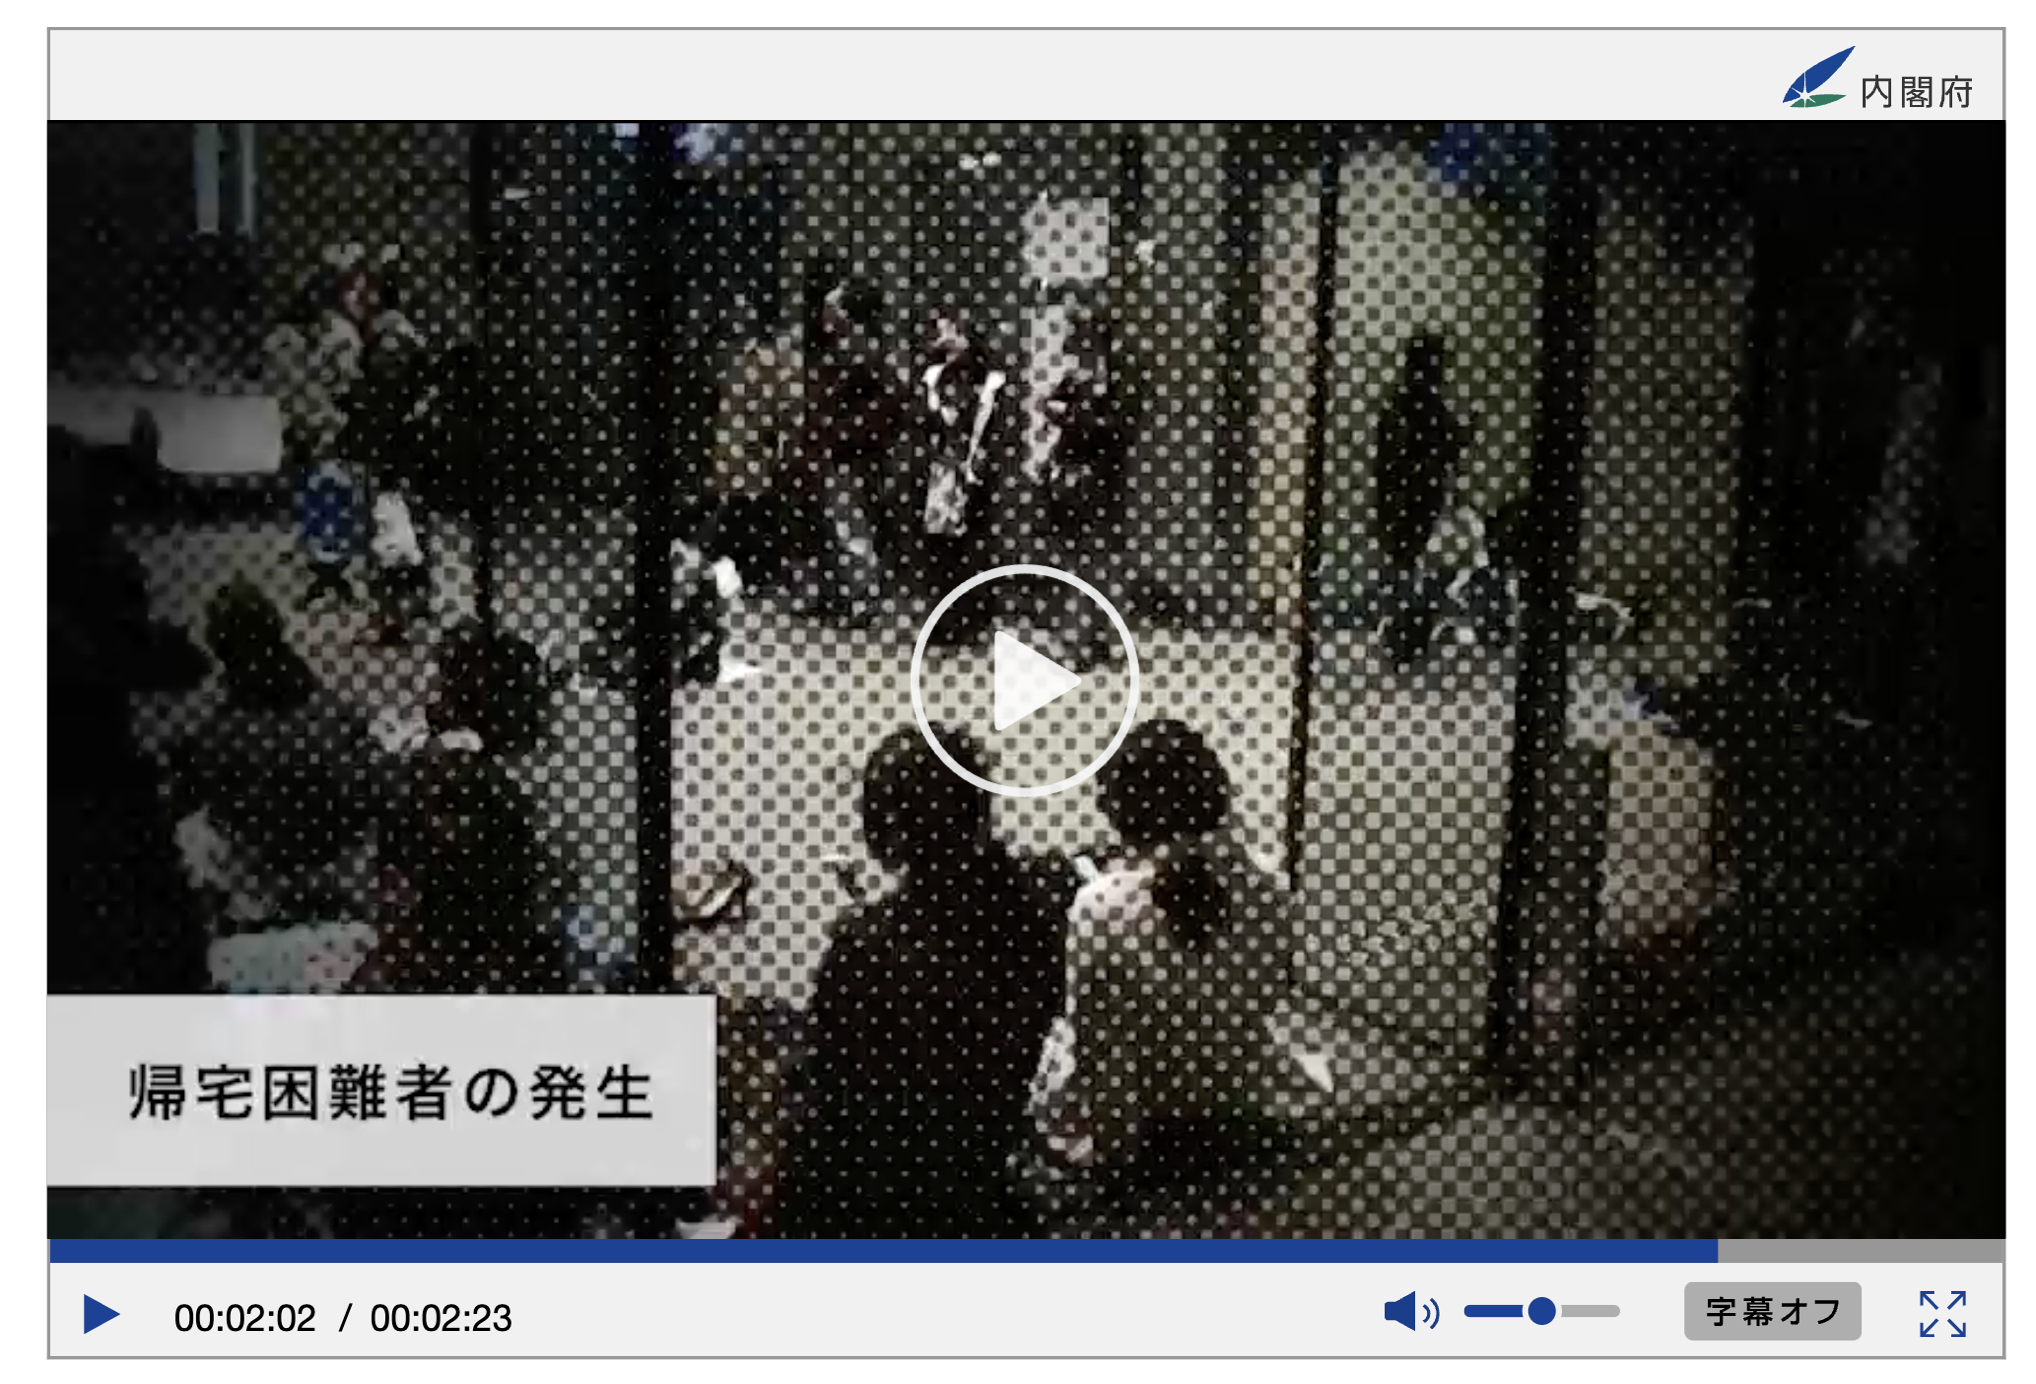
\includegraphics[width=\textwidth]{Figure/Figure5a.jpg}
    \caption{Difficulty in returning home}
    \label{fig5a}
  \end{subfigure}\hfill
  \begin{subfigure}{0.32\textwidth}
    \centering
    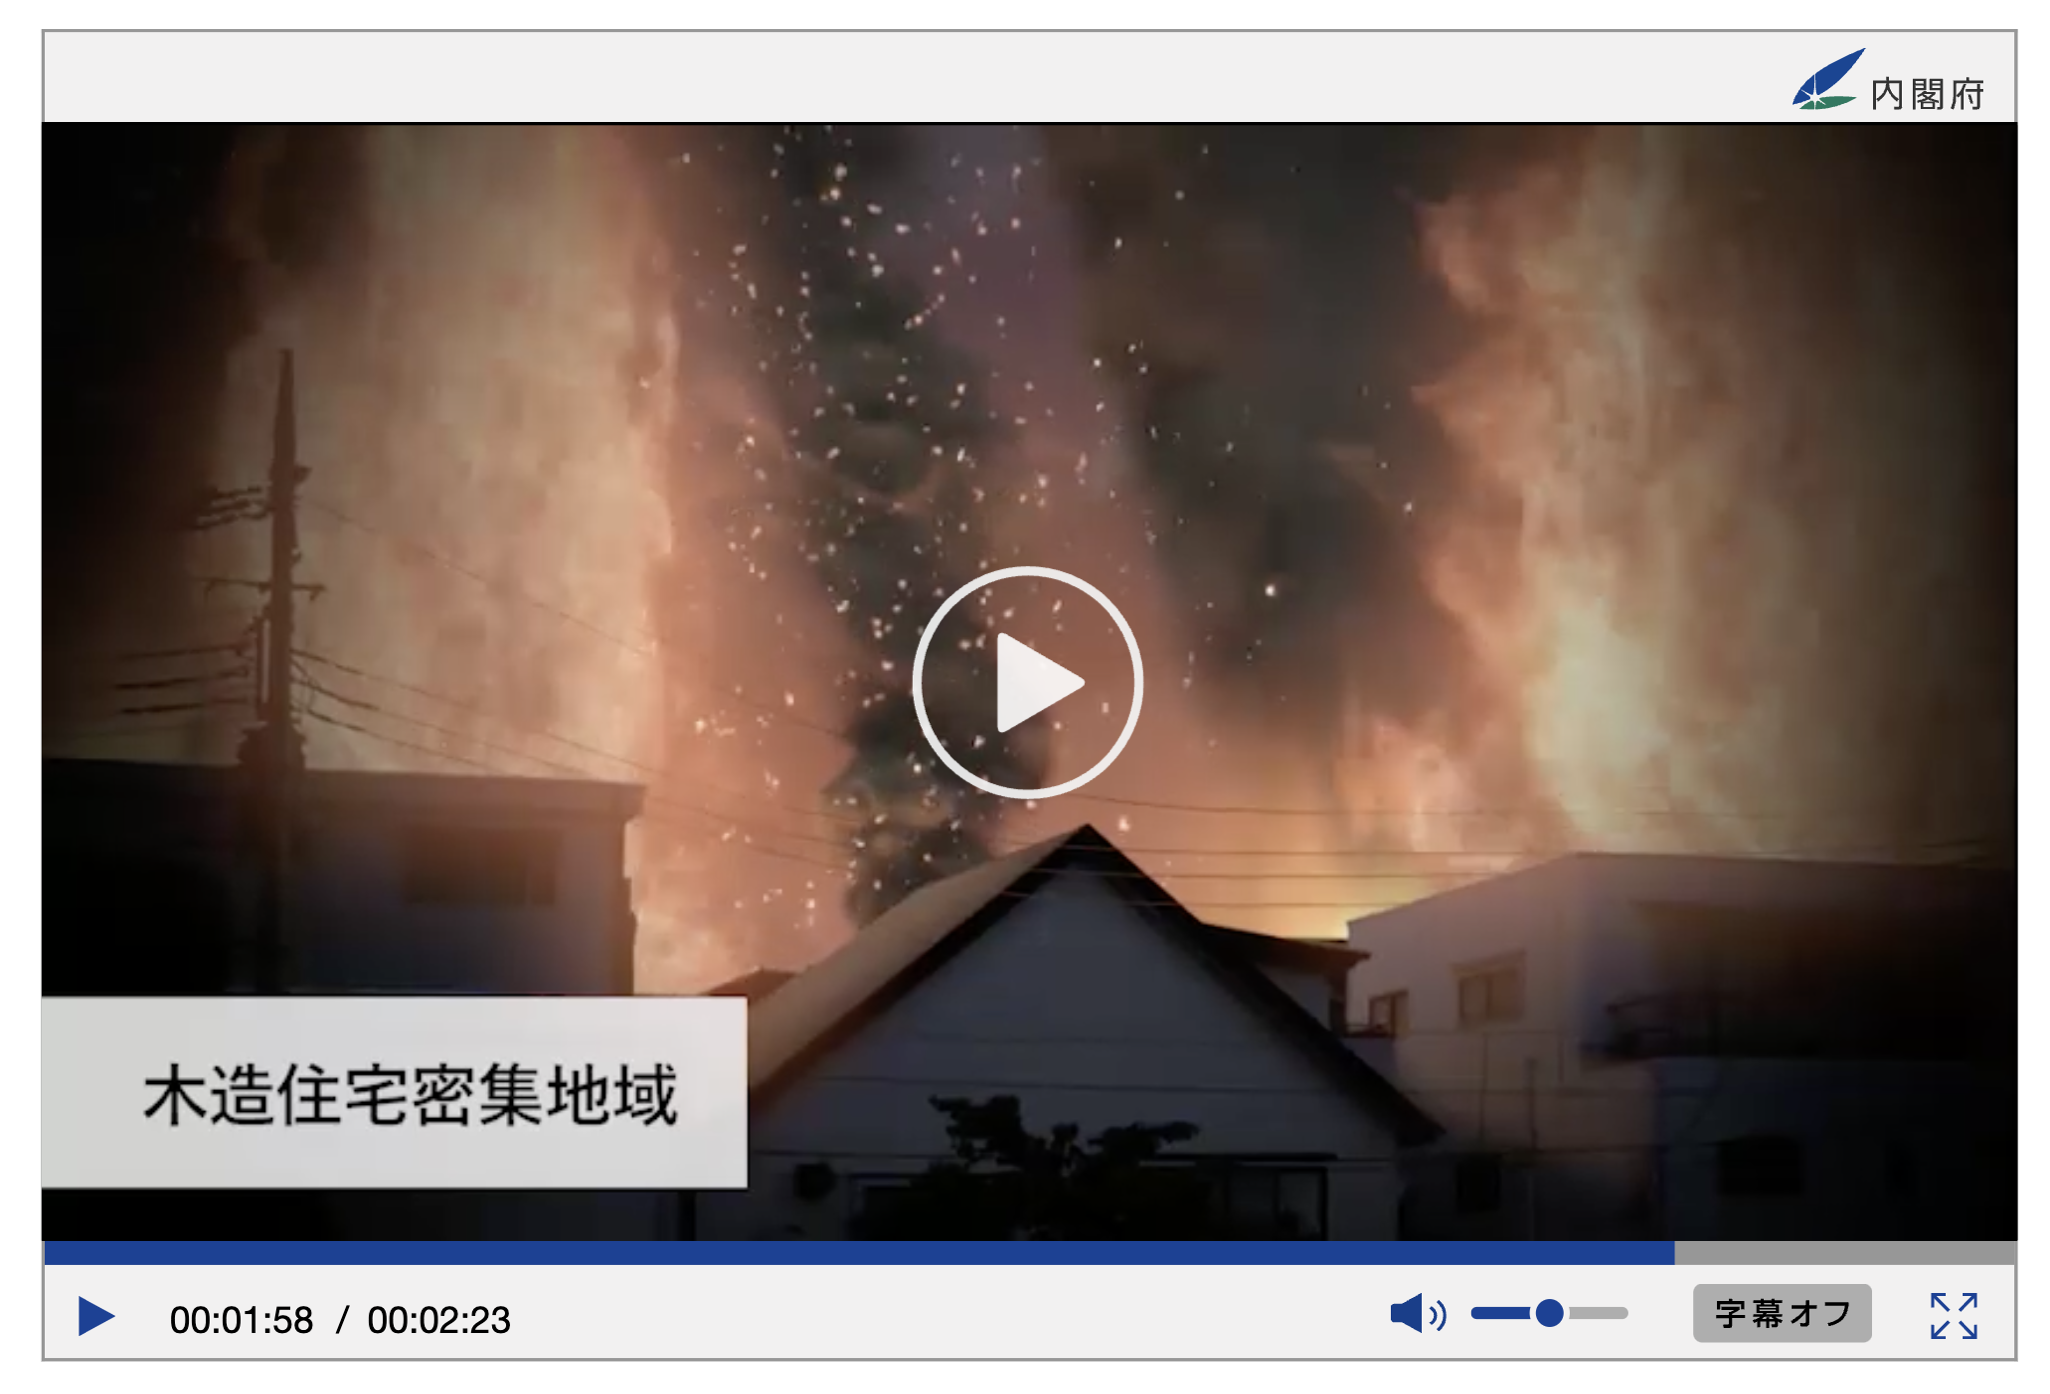
\includegraphics[width=\linewidth]{Figure/Figure5b.jpg}
    \caption{Dense area of wooden houses; Fire occurred easily}
    \label{fig5b}
  \end{subfigure}\hfill
  \begin{subfigure}{0.32\textwidth}
    \centering
    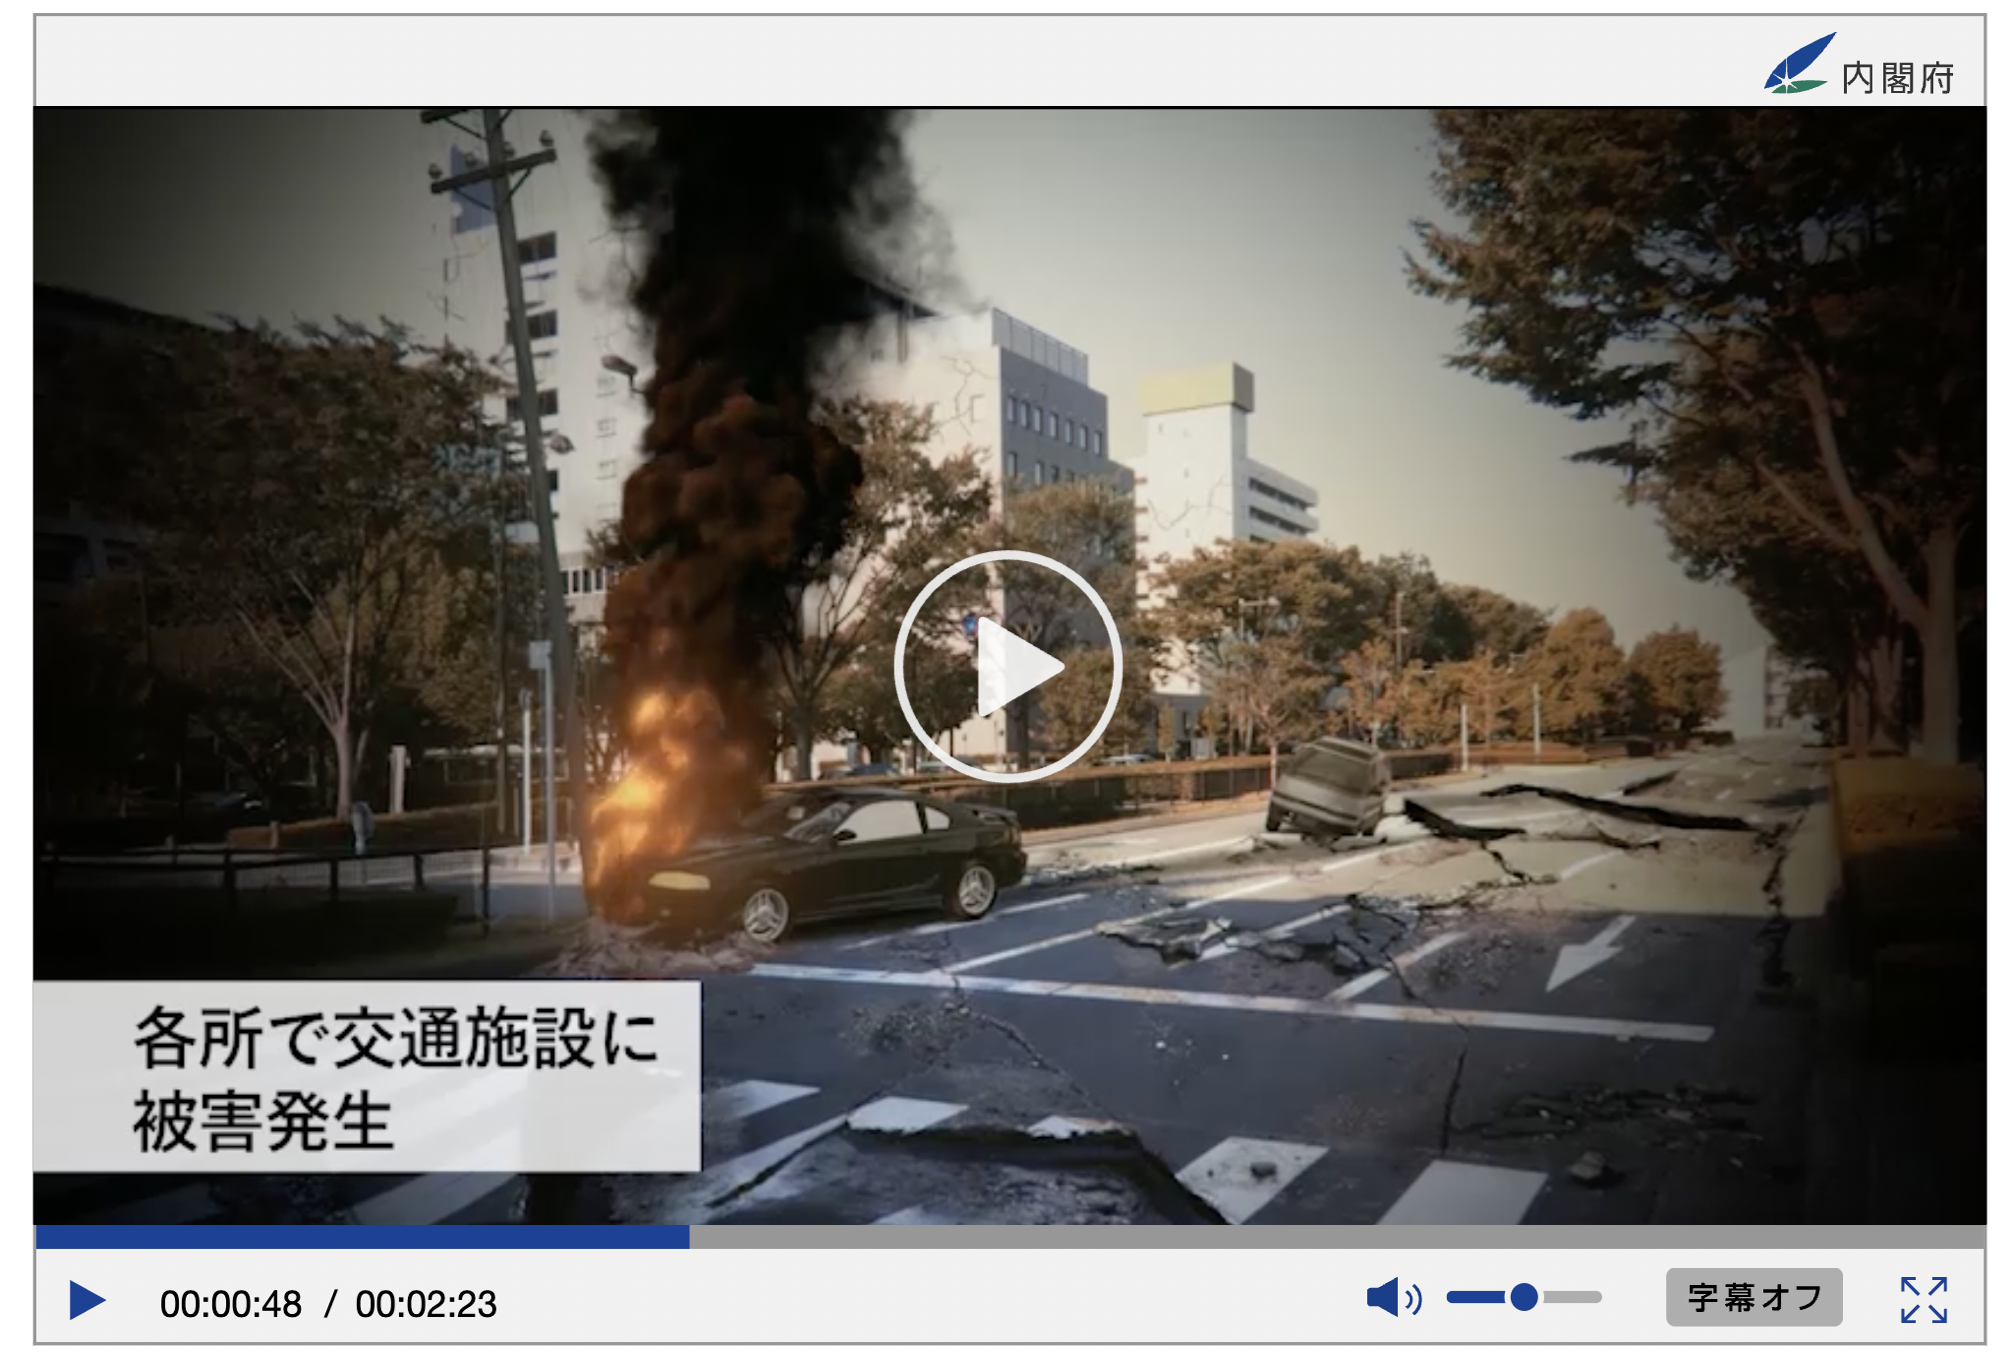
\includegraphics[width=\linewidth]{Figure/Figure5c.jpg}
    \caption{Damage to transportation facilities in many places}
    \label{fig5c}
  \end{subfigure}\hfill
  \begin{subfigure}{0.32\textwidth}
    \centering
    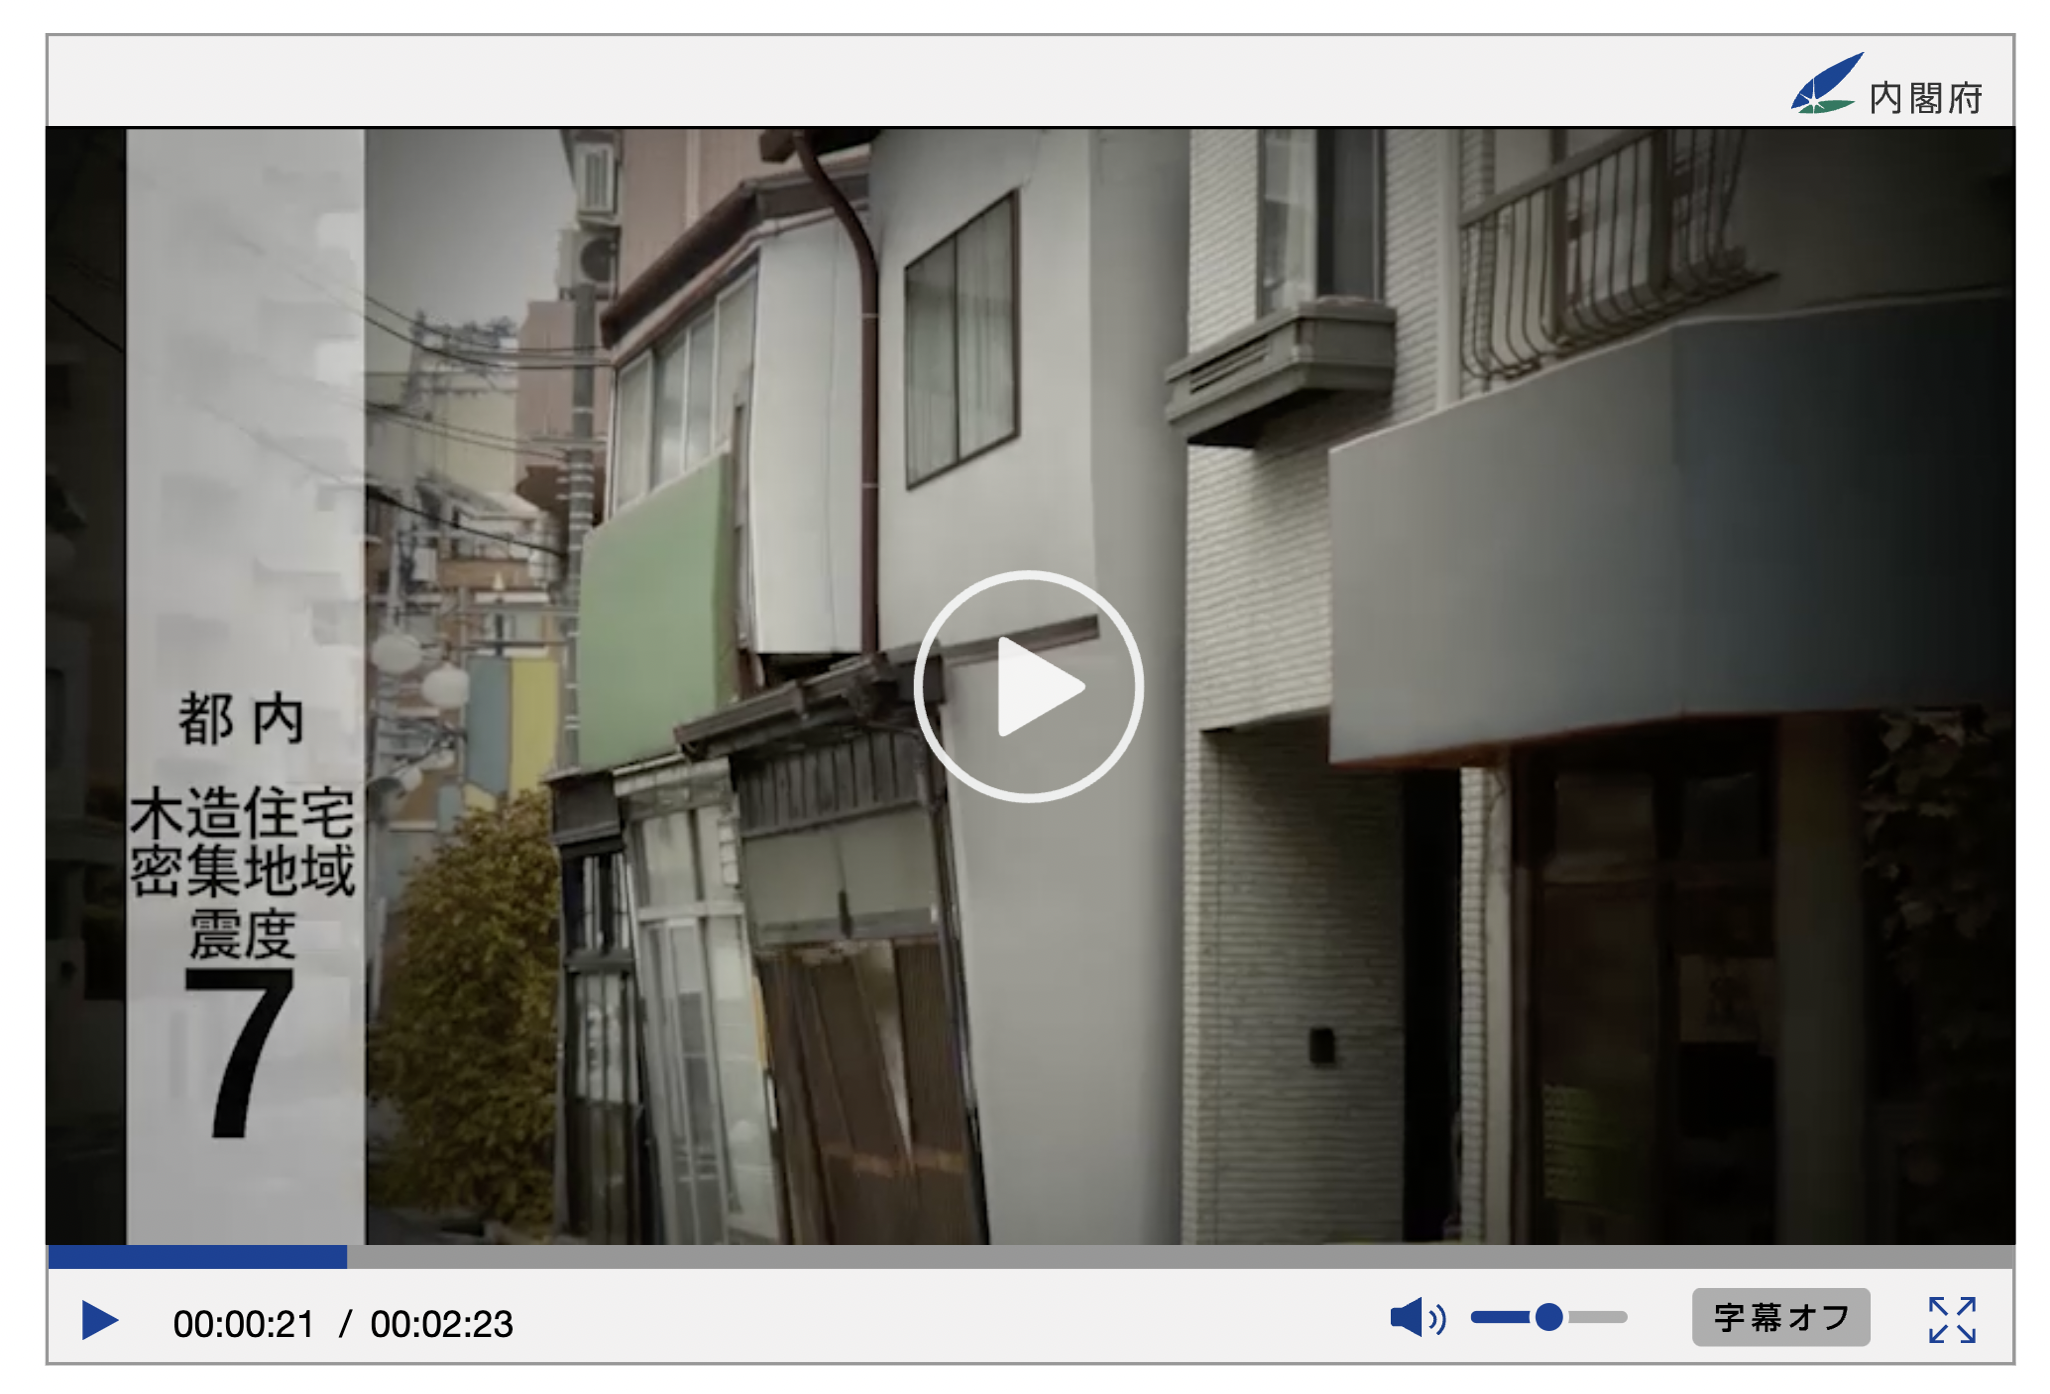
\includegraphics[width=\linewidth]{Figure/Figure5d.jpg}
    \caption{Tokyo-Wooden houses (Dense area); Seismic intensity 7}
    \label{fig5d}
  \end{subfigure}\hfill
  \begin{subfigure}{0.32\textwidth}
    \centering
    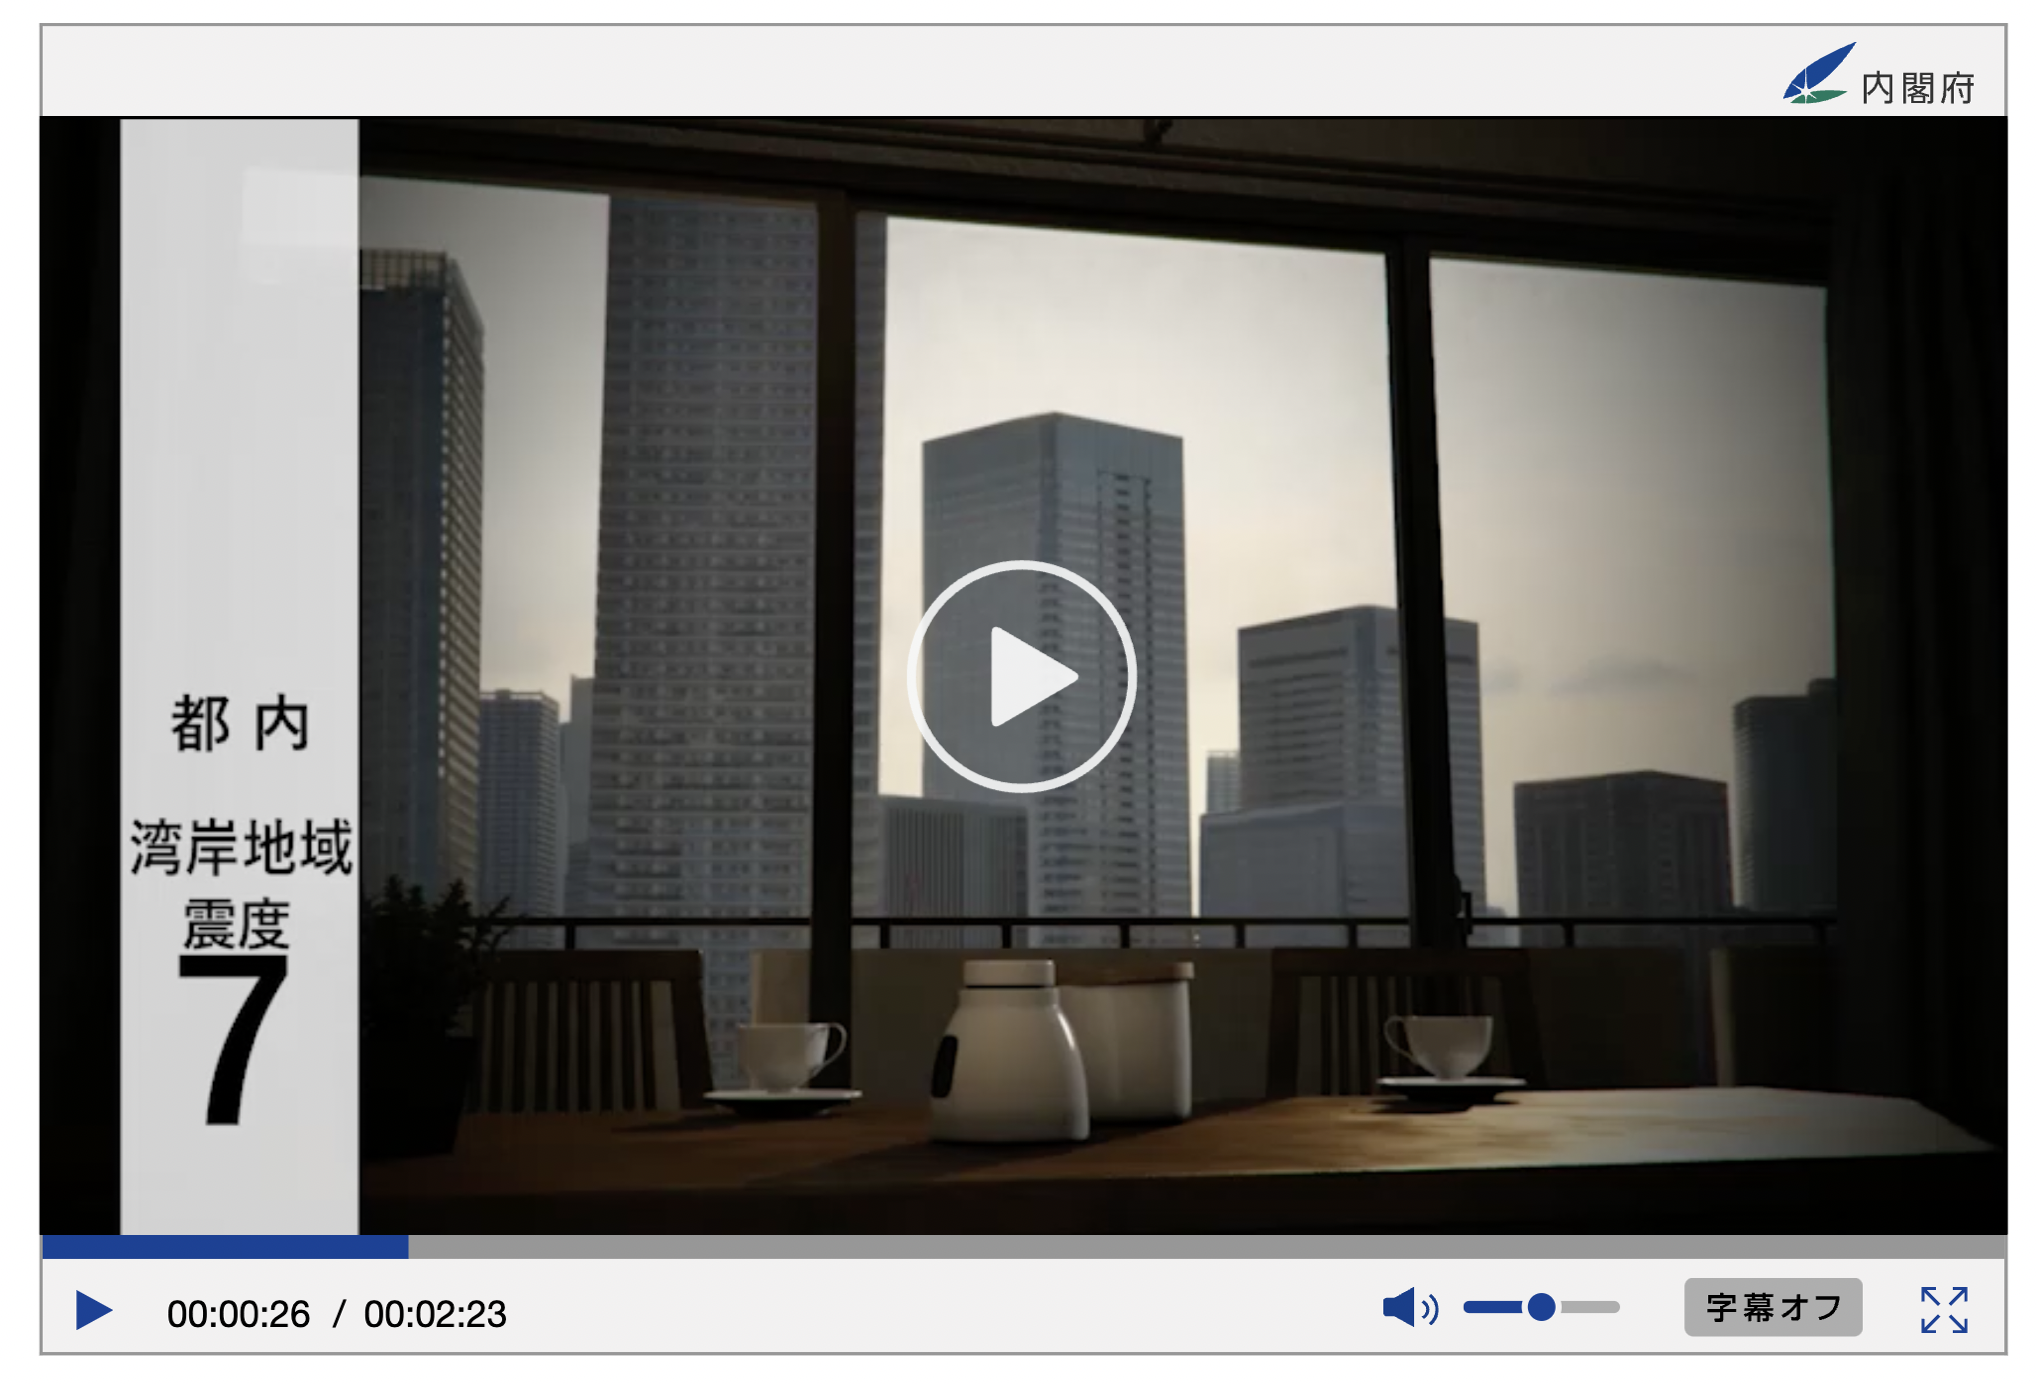
\includegraphics[width=\linewidth]{Figure/Figure5e.jpg}
    \caption{Tokyo-Bay Area; Seismic intensity 7}
    \label{fig5e}
  \end{subfigure}\hfill
  \begin{subfigure}{0.32\textwidth}
    \centering
    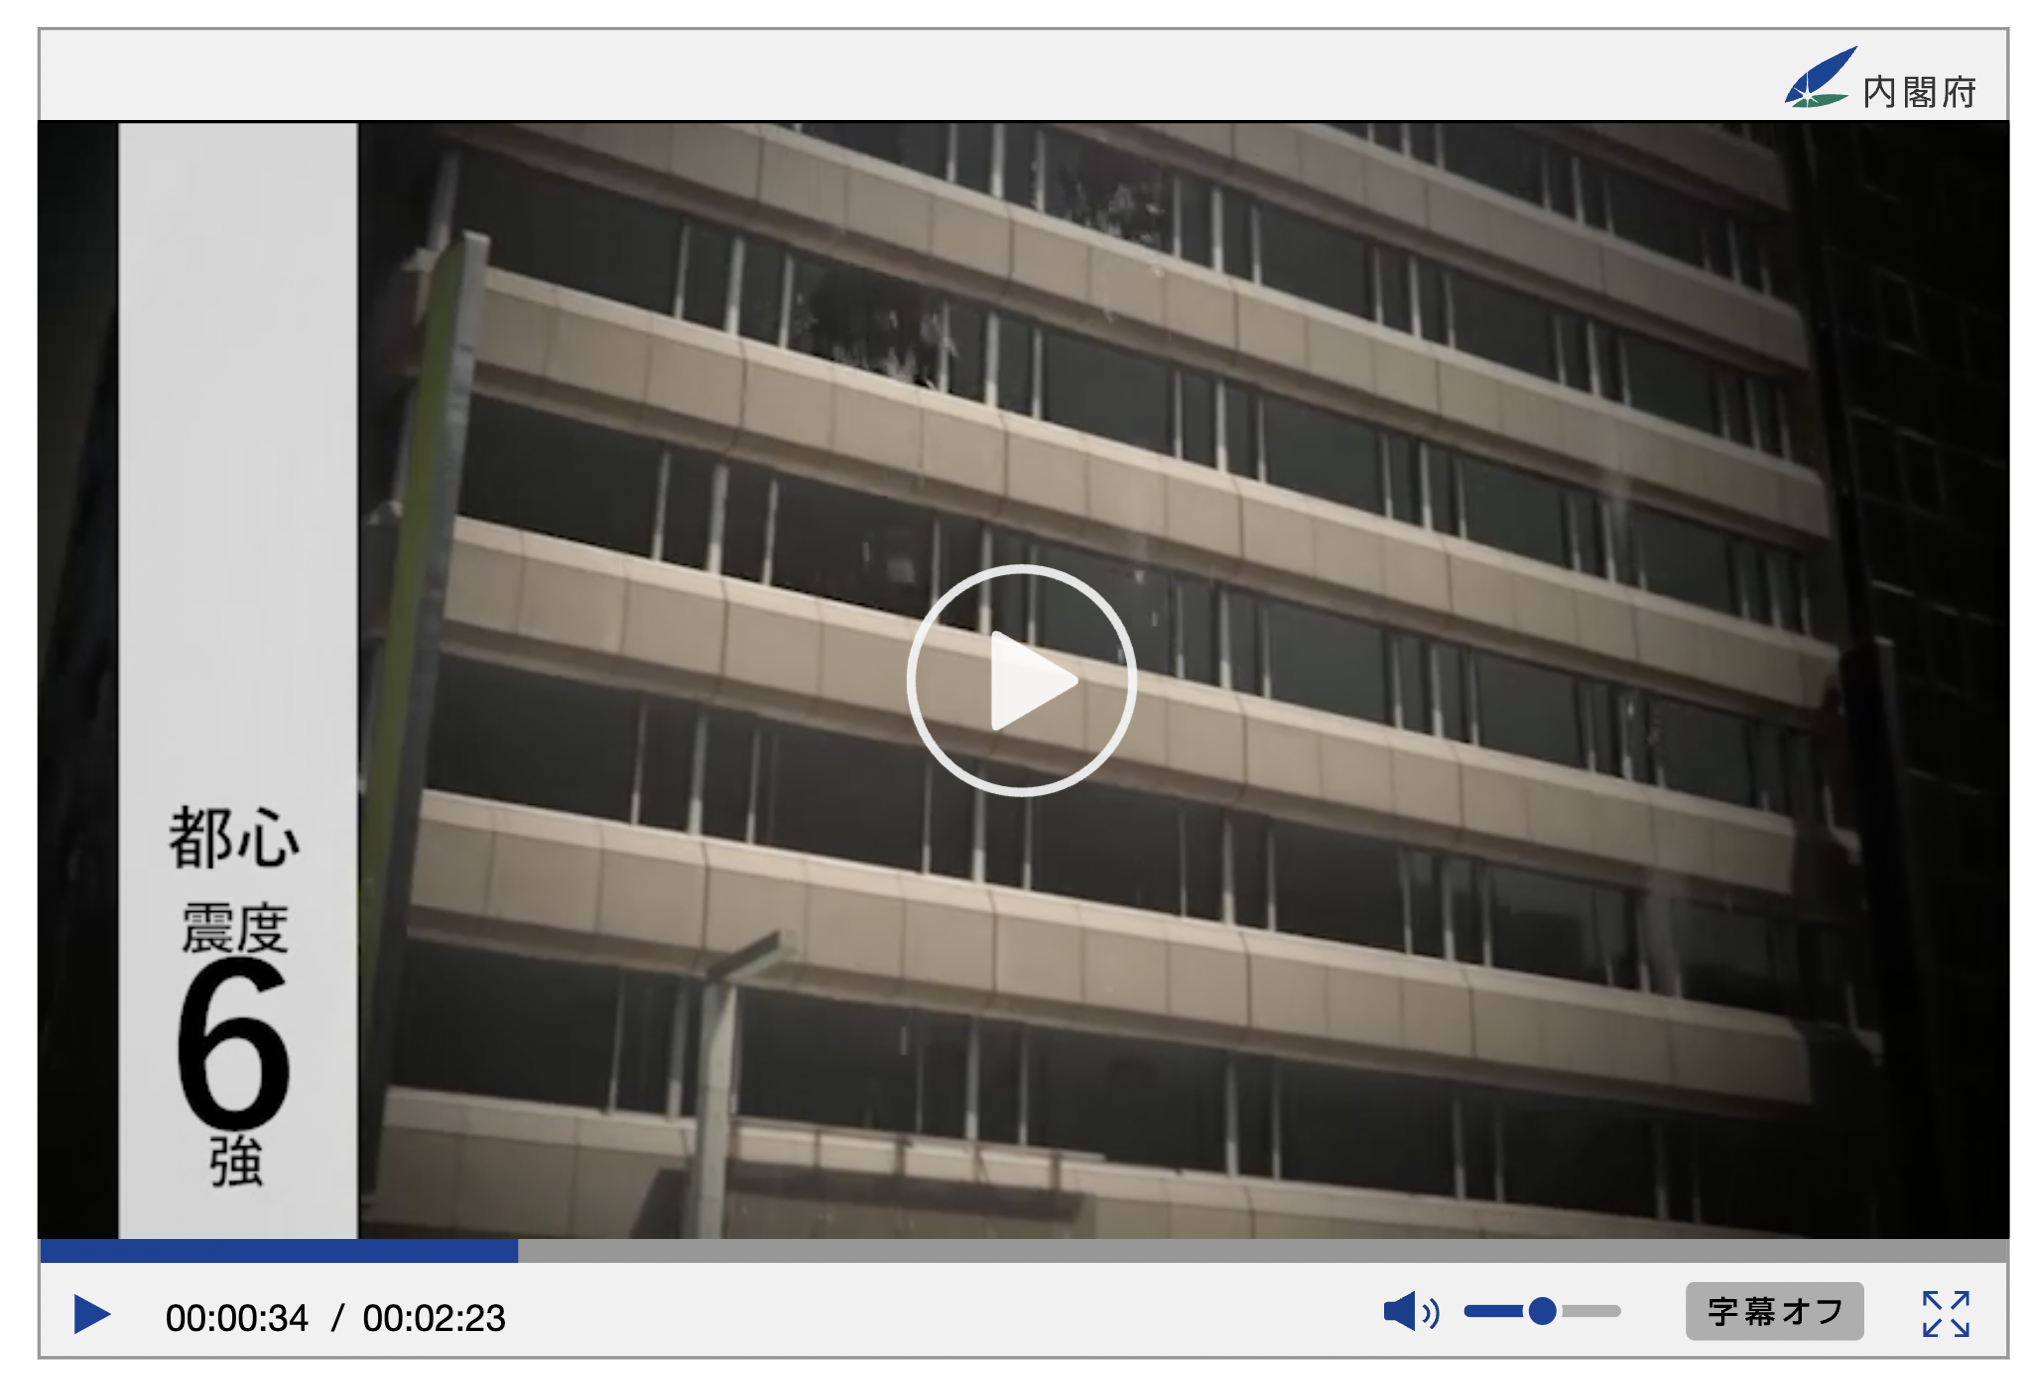
\includegraphics[width=\linewidth]{Figure/Figure5f.jpg}
    \caption{Tokyo; Seismic intensity 6-}
    \label{fig5f}
  \end{subfigure}
  \begin{subfigure}{0.32\textwidth}
    \centering
    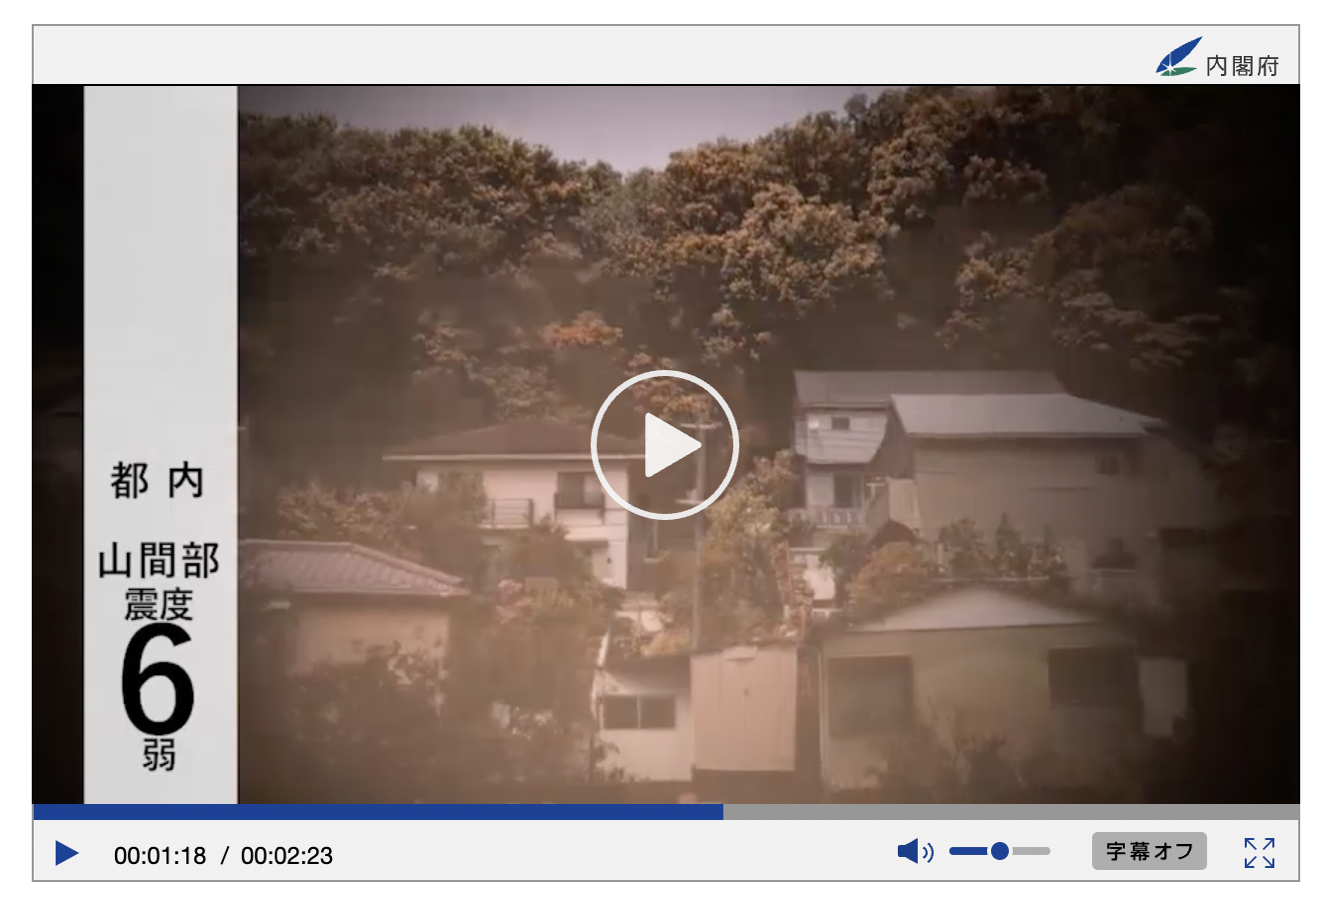
\includegraphics[width=\linewidth]{Figure/Figure5g.jpg}
    \caption{Tokyo-Mountainous region; Seismic intensity 6+}
    \label{fig5g}
  \end{subfigure}
  \centering
  \caption[Simulation video of  "Tokyo Metropolitan Earthquake".]{Simulation video of "Tokyo Metropolitan Earthquake".\protect\footnotemark }
  \label{fig5}
\end{figure*}
 \footnotetext{http://wwwc.cao.go.jp/lib\_012/syuto\_02.html}
%\fi


